\section{Zielsetzung}
Im diesem Versuch wird die Funktionsweise eines Geiger-Müller-Zählrohrs untersucht, indem die Totzeit, die Erholungszeit und die Charakteristik
eines Zählrohrs bestimmt wird. Außerdem soll die Abhänigkeit der Ladung von der Spannung geziegt werden.

\section{Theorie}
\subsection{Aufbau}
Der Aufbau eines Geiger-Müller-Zählrohrs ist in Abbildung \ref{abb:1} dargestellt. Hauptsächlich besteht dieses aus einem mit Gas gefüllten Hohlzylinder,
welcher als Kathode dient, und einem Anodendraht in der Mitte. Das Gas ist meist ein Gemisch aus Argon und Ethylalkohol. Wird nun eine Spannung an das
Geiger-Müller-Zählrohr angelegt ensteht ein radialsymmetrisches elektrisches Feld im Inneren des Rohrs, welches beschrieben wird durch
\begin{equation*}
  E(r) = \frac{U}{\symup{ln}(r_k/r_a)} \cdot \frac{1}{r} \ ,
\end{equation*}
wobei $r_k$ den Radius des Hohlzylinders, $r_a$ den Radius des Anodendrahtes und $U$ die anliegende Spannung beschreibt. Da mit dem Geiger-Müller-Zählrohr
vor allem $\alpha$- und $\beta$-Strahlung nachgwiesen werden kann und diese aber von dem Hohlzylinder absorbiert werden würden, ist das Eintrittsfenster aus
Mylar-Folie, welches sogar auch $\alpha$-Strahlung hindurch lässt.
\begin{figure}
  \centering
  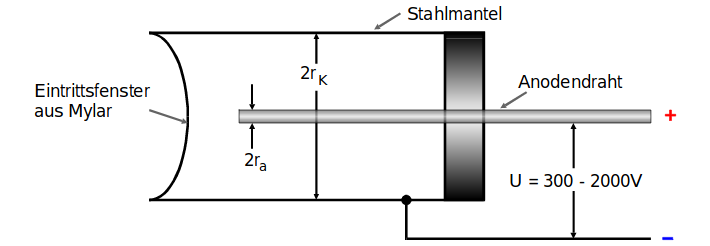
\includegraphics[scale=0.5]{a.png}
  \caption{Aufbau eines Geier-Müller-Zählrohrs. \cite{Q1}}
  \label{abb:1}
\end{figure}

\subsection{Funktionsweise}
In einem Geiger-Müller-Zählrohr kann $\alpha$- und $\beta$-Strahlung zu fast \SI{100}{\percent} nachgewiesen werden, $\gamma$-Stahlung hingegen ist zu hochenergetisch, hier kann nur
Strahlung mit hohen Intensitäten nachgewiesen werden, da die Wechselwirkung mit Materie hier relativ gering ist.
Gelangt nun ein geladenens Teilchen in das Volumen des Geiger-Müller-Zählrohrs, führt dies dazu, dass ein Teilchen aus dem Gas ionisiert wird. Die
Ionisation führt dazu, dass ein Kation und ein Elektron entstehen: Das Elektron wird durch das elektrische Feld in Richtung des Anodendrahtes beschleunigt
und dort absorbiert. Der daraus entstehende Elektrische Impuls wird durch einen Kondensator ausgekoppelt und verstärkt, sodass ein Zähler die Impulse messen kann.
Das Kation hingegen wird in Richtung des Kathodenzylinders beschleunigt und eigentlich im Kathodenmaterial absorbiert. Hierbei ist
aber zu beachten, dass das Kation eine hohe Energie hat und somit aus dem Kathodenmaterial weitere Elektronen herauslösen kann, diese werden
als \textbf{Sekundärelektronen} bezeichnet. Würde dieser Effekt nicht verhindern werden, würden diese Elektronen zu einem weiteren Ausschlag des Geiger-Müller-Zählrohrs
führen. Dieser Effekt kann aber durch Hinzugabe von Ethylalkoholgas verhindert werden, denn die Kationen werden von diesen Atomen absorbiert und regen diese
zu Schwingungen an. Somit gelangen die Kationen nicht mehr bis zu dem Kathodenmaterial und können auch somit keine Sekundärelektronen mehr herauslösen.
Da die Energie des eintreffenden, geladenen Teilchens viel höher ist, als die Ionisierungsenergie, können mehrere Ionisationen gleichzeitig stattfinden.
Der weitere Verlauf nach der Ionisierung hängt stark von der angelegten Spannung ab:
\begin{itemize}
  \item Für niedrige Spannungen (siehe Abbildung \ref{abb:2}, Bereich I) ist die Wahrscheinlichkeit einer \textbf{Rekombination} sehr hoch. Durch die Rekombination
  wird die Ionisation rückgängig gemacht. Es enstehen in diesem Bereich also nur sehr geringe, kaum messbare Ströme.
  \item Im Proportionalitätsbereich (siehe Abbildung \ref{abb:2}), Bereich II und III) regt die oben beschriebene Ionisation weiter Ionisationen an, indem
  das ionisierte Elektron durch das elektrische Feld in Richtung des Anodendrahtes beschleunigt wird. Hierbei gewinnt es so viel Energie, dass
  es ein weiteres Atom zu Ionisierung anregen kann. So ensteht schnell eine \textbf{Elektronenlawine}. Wichtig in diesem Bereich ist außderdem, dass die gemessenen
  elektrischen Impulse proportinal zu der \textbf{Energie} und der \textbf{Intensität} der eindringenden Strahlung ist.
  \item In dem Spannungsbereich des Geiger-Müller-Zählrohrs (siehe Abbildung \ref{abb:2}, Bereich IV) kommt zu der Elektronenlawine noch ein weiter Effekt hinzu:
  Bei der Elektronenlawine enstehen nicht nur eine große Anzahl an Elektronen, sondern für hohe Spannungen auch \textbf{UV-Photonen}. Diese können, aufgrund ihrer
  neutralen Ladung, auch senkrecht oder entgegengesetzt der Feldlinien in dem Zylinderkondensator bewegen und somit weitere Atome und somit Elektronenlawinen anregen.
  In diesem sogenannten \textbf{Auslösebereich} ist der gemessene elektrische Impuls jetzt nurnoch von der \textbf{Intensität} abhängig und es kann keine Aussage mehr
  über die Energie der Strahlung getroffen werden.
  \item Wird der Auslösebereich überschritten und die Spannung weiter erhöht, so wird durch eine einzelne Ionisation eine Dauergasentladung enzündet und
  das Geiger-Müller-Zählrohr wird durch daraus entstehende zu hohe Stromdichten zerstört. Dies wird der Bereich der \textbf{selbständigen Gasentladung} genannt.
\end{itemize}
\begin{figure}
  \centering
  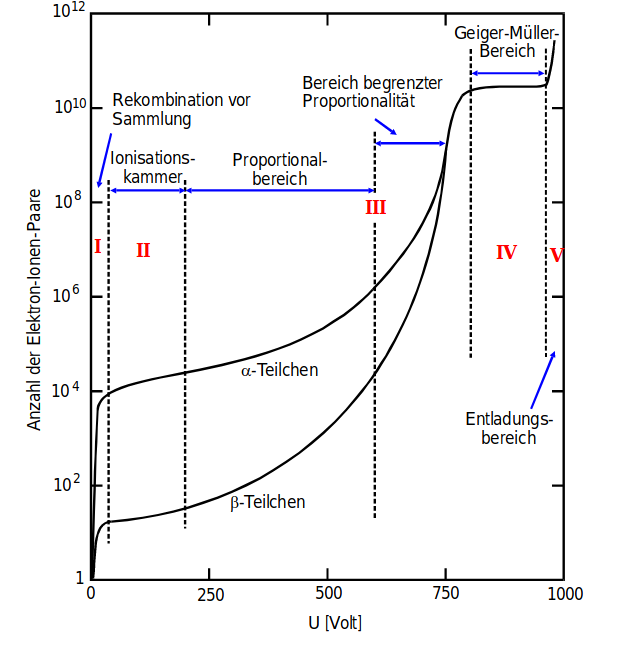
\includegraphics[scale=0.4]{b.png}
  \caption{Anzahl Elektronen in Abhängigkeit der Spannung. \cite{Q1}}
  \label{abb:2}
\end{figure}

\subsection{Totzeit und Erholungszeit}
Im Gegensatz zu Elektronen, die sich durch ihre geringe Masse relativ schnell zum Anodendraht bewegen, werden die positiv geladenen Kerne durch ihre größere Masse
langsamer beschleunigt und benötigen für die Zeit bis zur Kathode länger. Da diese nicht instantan zum Kathodenmaterial gelangen, bildet sich für eine kurze Zeit eine
positive Raumladung, auch \textbf{Ionenschlauch} genannt, welche sich dem elektrischen Feld entgegensetzt. Das führt dazu, dass in dem Bereich um den Anodendraht
keine Ionisationen mehr möglich sind. Also auch wenn in diesem Zeitraum ein weiteres geladenenes Teilchen in das Zählrohrvolumen eintritt, kann dies nicht detektiert werden.
Es wird also eine Zeit $T$ definiert, in der es nach einer Detektion nicht möglich ist, weitere Teilchen zu detektieren, die sogenannte \textbf{Totzeit}.
Nach solch einer Ionisationslawine und der Totzeit müssen die Ionen zunächst wieder vollständig neutralisiert werden, damit das elektrische Feld nicht mehr durch
Ionen gestört werden kann. Diese Zeit wird \textbf{Erholungszeit} genannt.
Diese beiden charakteristischen Zeiten können an einem OSzilloskop durch Darstellung des elektrischen Impulses abgelesen werden. Außerdem gibt es für die Messung der
Totzeit noch die \textbf{Zwei-Quellen-Methode}: Hierbei wird in einem Zeitintervall eine Messung mit der Quelle $Q_1$ durchgeführt, darauf folgend eine Messung im selben
Zeitintervall mit der Quelle $Q_1$ und $Q_2$ und zuletzt eine Messung mit der Quelle $Q_2$. Hierbei sollten sich die jeweiligen Quellen zu den Messungen an der selben
Stelle befinden. Das Ergebnis dieser Messungen wird hervorbringen, dass gilt
\begin{equation*}
  N_{\symup{1+2}} < N_1 + N_2
\end{equation*}
wobei $N$ jeweils die Anzahl der Counts ist.
Aus dieser Relation kann näherungsweise die Totzeit $T$ bestimmen werden durch
\begin{equation}
  \label{eq:Totzeit}
  T \approx \frac{N_1+N_2-N_{\symup{1+2}}}{2N_1N_2}
\end{equation}
Die Totzeit und die Erholungszeit sind in Abbildung \ref{abb:3} dargestellt.
\begin{figure}
  \centering
  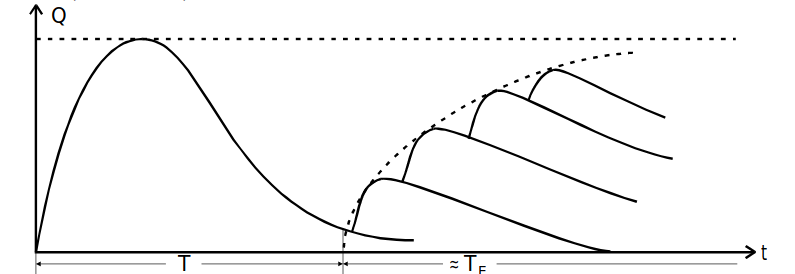
\includegraphics[scale=0.4]{c.png}
  \caption{Totzeit und Erholungszeit eines Geiger-Müller-Zählrohrs. \cite{Q1}}
  \label{abb:3}
\end{figure}


\subsection{Charakteristik eines Zählrohrs}
Die Charakteristik eines Geiger-Müller-Zählrohr wird bei konstanter Intensität aufgenommen, hierzu wird die Spannung gegen die erfasste Teilchenanzahl aufgetragen.
Solch eine Charakteristik ist in Abbildung \ref{abb:4} zu sehen.
\begin{figure}
  \centering
  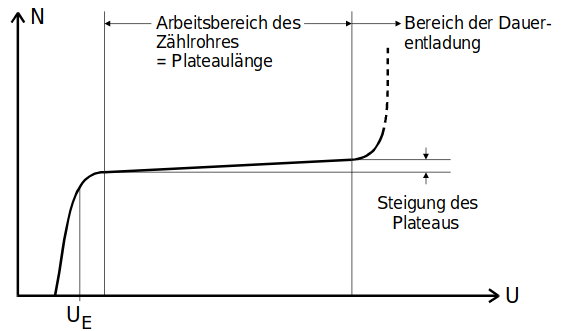
\includegraphics[scale=0.5]{d.png}
  \caption{Charakteristik eines Geiger-Müller-Zählrohrs. \cite{Q1}}
  \label{abb:4}
\end{figure}
Etwa nach der Spannung $U_E$ setzt der Auslösebereich ein, hier beginnt bei der Charakteristik das Plateau. Dieses Plateau hat idealerweise keine Steigung, dies kann aber
aufgrund von Nachentladungen nicht erreicht werden. Je geringer die Stigung und je länger das Plateau, desto höher ist die Qualität des Geiger-Müller-Zählrohrs.
Nach dem Plateau schließt sich der Bereich der Dauerentladung an, hierbei kann das Zählrohr für hohe Spannungen zerstört werden.

\subsection{Messung der pro Teilchen vom Zählrohr freigesetzten Ladungsmenge}
Durch den mittleren Zählrohrstrom $\bar{I}$ kann außerdem die Ladung $\Delta Q$ berechnet werden, hierzu werden die Definitionen
\begin{align*}
  \bar{I} &= \int_0^{\tau} \frac{U(t)}{R} \symup{d}t \\
  \bar{I} &= \frac{\symup \Delta Q}{\symup \Delta t} \, Z
\end{align*}
gleichgesetzt, wobei $U(t)$ die Spannung, $R$ der Widerstand, $\symup \Delta t$ das Zeitintervall, $\symup \Delta Q$ die in dem Zeitintervall $\symup \Delta t$
gemessene Ladung und $Z$ die Anzahl der registrierten Teilchen beschreibt.

\section{Durchführung}
Der Versuch wird nach Abbildung \ref{abb:5} aufgebaut. Zur Messung wird ein $\beta$-Stahler vor dem Geiger-Müller-Zählrohr platziert.

\begin{figure}
  \centering
  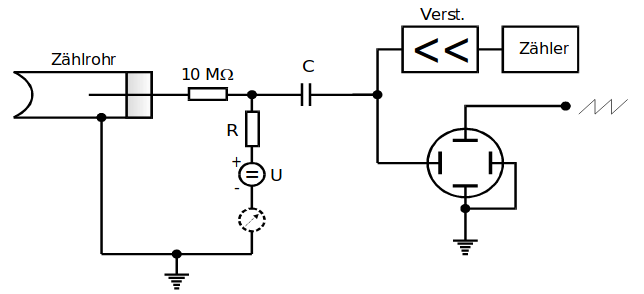
\includegraphics[scale=0.5]{e.png}
  \caption{Versuchsaufbau. \cite{Q1}}
  \label{abb:5}
\end{figure}

Zur Messung der Charakteristik des Geiger-Müller-Zählrohrs werden die Counts in Abhängigkeit der Spannung gemessen. Hierbei wird ein Bereich von
\SI{300}{\volt} bis \SI{700}{\volt} in \SI{10}{\volt}-Schritten abgetastet und die jeweiligen Counts in einer Zeit von $\Delta t = \SI{60}{\second}$ gemessen.

Im zweiten Teil des Versuch soll die Totzeit $T$ und die Erholungszeit $T_{\symup{er}}$ gemessen werden. Hierzu werden die elektrischen Impulse auf dem Oszilloskop
sichtbar gemacht und durch den Trigger an einer Stelle zum Stehen gebracht. Nun wird die Totzeit an abgelesen, indem die Breite des Impulses abgelesen wird.
Die Erholungszeit kann dadurch bestimmt werden, dass die Zeit zwischen dem Ende des Hauptimpulses und dem Anfang des nächsten Impulses gemessen wird, welcher
genauso hoch sein muss, wie der Hauptimpuls. An der Stelle haben sich die Ionen wieder vollständig neutralisiert und es kann ein neuer Impuls gemessen werden.
Diese Messungen werden für 5 verschiedene Spannungen im bereich des Plateaus durchgeführt.

Zur genaueren Messung der Totzeit wird außerdem die Zwei-Quellen-Methode einmal durchgeführt, indem je beide Quellen einzeln und einmal beide Quellen zusammen
in einem Zeitintervall von \SI{60}{\second} gemessen werden. Die Spannung beträgt hierbei \SI{550}{\volt}.

Zuletzt soll die Abhängigkeit der Ladung von der Spannung bestimmt werden, hierzu werden für mindestens 5 verschiedene Spannungen zwischen \SI{300}{\volt} und
\SI{700}{\volt} die Counts und die Stromstärke gemessen.

\section{Auswertung}
\subsection{Charakteristik des Geiger-Müller-Zählrohrs}
Im ersten Teil des Versuchs wird die Charakteristik des Geiger-Müller-Zählrohrs untersucht. Hierzu
wird die Zählrate $N$ gegen die Betriebsspannung U aufgetragen. Die zur Erstellung des Plots \ref{abb1}
benötigten Werte befinden sich ins Tabelle \ref{tab1}. Die Ausschläge des Geiger-Müller-Zählrohrs unterliegen
der Poissonverteilung und sind somit fehlerbehaftet. Dieser statistische Fehler wird durch die Fehlerbalken
in der Graphik \ref{abb1} gekennzeichnet und berechnet sich mit $\sqrt{\symup{N}}$.
Im Plot ist zwischen \SI{370}{\volt} und \SI{610}{\volt} deutlich ein Plateau zu erkennen, welches eine Breite
von \SI{240}{\volt} aufweist. Durch die Werte der Plateaus wird eine lineare Ausgleichsgerade gelegt, die in Abbildung \ref{abb2} explizit zu sehen ist,
die folgende Gestalt aufweist:
\FloatBarrier
\begin{align*}
  F = ax + b
\end{align*}
\FloatBarrier
Hierbei ergeben sich für $a$ und $b$ folgende Werte:
\FloatBarrier
\begin{align*}
  a &= \SI{0.021(5)}{} \\
  b &= \SI{182,7(27)}{\frac{1}{s}}\\
\end{align*}
\FloatBarrier
Mit Hilfe folgender Formel lässt sich dann der Steigungswinkel \alpha mit zugehörigem Fehler berechnen:
\begin{align*}
  \alpha &= \symup{arctan}(a) = \SI{1,203}{\degree} \\
  \Delta \alpha &= \sqrt{\left( \frac{1}{a^2 + 1} \Delta a \right)^2 } = \SI{0,002}{\degree}
\end{align*}
\FloatBarrier
Folglich wird eine Steigung von \SI{2,1(002)}{\percent} pro \SI{100}{\volt} mit Hilfe folgender Formeln berechnet:
\FloatBarrier
\begin{align*}
  S_{\symup{\si{\percent}}} &= \symup{tan}(\alpha) \cdot 100 \\
  \Delta S_{\symup{\si{\percent}}} &= \sqrt{\left( \frac{1}{\symup{cos}^2(a)} \Delta \alpha \right)^2}
\end{align*}.
\FloatBarrier

\begin{table}
  \centering
  \caption{Messwerte zur Erstellung des Plots zur Analyse der Charakteristik des Geiger-Müller-Zählrohrs.}
  \begin{tabular}{ c c c c }
  \toprule
  {U / V} & { N } & { U / V } & { N } \\
  \midrule
300   &       0   &   510   &   11665   \\
310   &   10509   &   520   &   11647   \\
320   &   10938   &   530   &   11658   \\
330   &   11256   &   540   &   11811   \\
340   &   11253   &   550   &   11737   \\
350   &   11261   &   560   &   11479   \\
360   &   11367   &   570   &   11839   \\
370   &   11476   &   580   &   11621   \\
380   &   11279   &   590   &   11642   \\
390   &   11367   &   600   &   11697   \\
400   &   11624   &   610   &   11570   \\
410   &   11298   &   620   &   11724   \\
420   &   11436   &   630   &   11628   \\
430   &   11617   &   640   &   11844   \\
440   &   11668   &   650   &   11929   \\
450   &   11468   &   660   &   11861   \\
460   &   11609   &   670   &   12040   \\
470   &   11409   &   680   &   12279   \\
480   &   11677   &   690   &   12236   \\
490   &   11599   &   700   &   12388   \\
500   &   11665   &         &           \\
    \bottomrule
  \end{tabular}
  \label{tab1}
\end{table}
\FloatBarrier

\begin{figure}
  \centering
  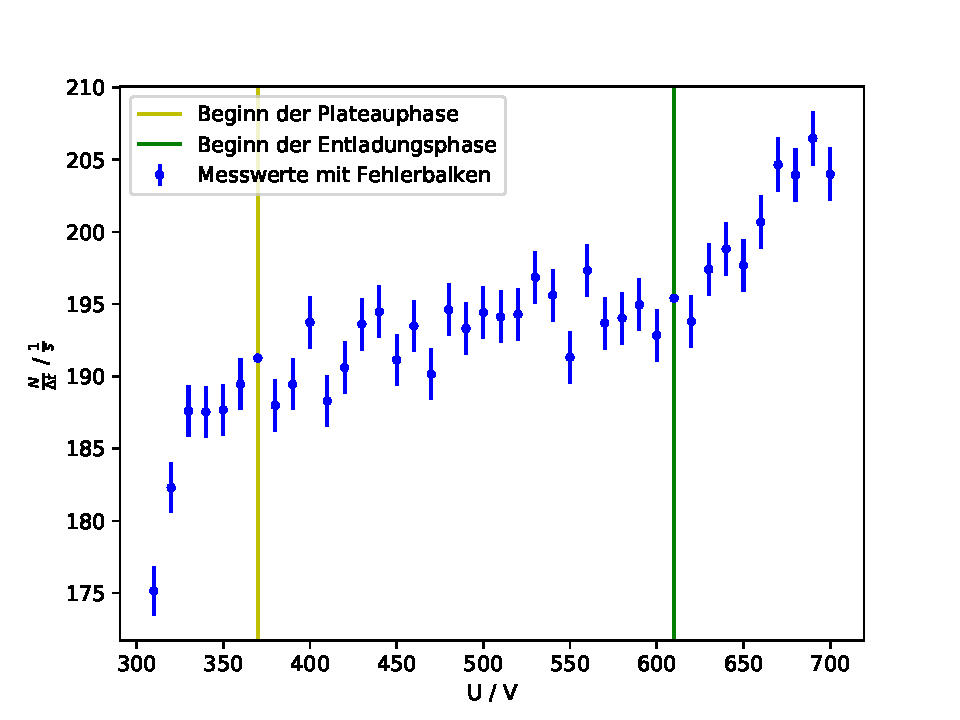
\includegraphics[scale=0.5]{1.pdf}
  \caption{Plot zur Untersuchung der Charakteristik des Geiger-Müller-Zählrohrs.}
  \label{abb1}
\end{figure}
\FloatBarrier
\begin{figure}
  \centering
  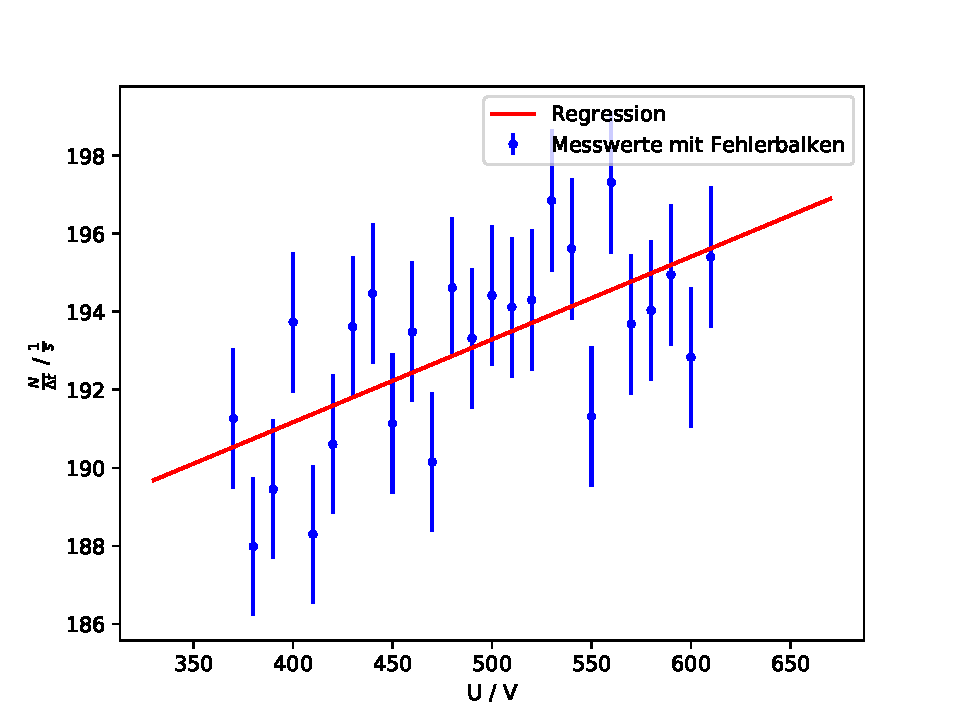
\includegraphics[scale=0.5]{1b.pdf}
  \caption{Plot zur Analyse des Plateaubereichs mit eingezeichnetem linearem Fit.}
  \label{abb2}
\end{figure}
\FloatBarrier
\subsection{Qualitative Bestimmung der Tot- sowie der Erholungszeit}
Die Totzeit kann auf zwei Arten ermittelt werden. Zum einen können die einlaufenden Impulse
mittels eines Oszilloskops sichtbar gemacht werden. Dann kann leicht der Abstand zwischen
Beginn der Kurve und dem Erreichen der Nullinie abgelesen werden. Hier ergab sich für verschiedene
Betriebsspannungen eine mittlerer Wert von $T_{\symup{T}}$=$\SI{207,5(95)}{\micro \second}$. Außerdem kann
auf ähnliche Weise die Erholungszeit ermittelt werden. Hierzu wird der Oszillograph genau beobachtet,
Da in dessen Display für kurze zeit Kurven mit der gleichen Höhe wie die der Totzeit in einem gewissen Abstand
zu dieser aufflackern. Der Abstand zwischen dem Maximum der Kurve der Totzeit und dem Maximum der Erholungszeit
wird ebenfalls für verschiedene Betriebsspannungen abgelesen, gemittelt und im Anschluss dazu der Fehler berechnet,
was zu einem Wert für die Erholungszeit ($T_{\symup{E}}$) von $\SI{0,525(96)}{\milli \second}$ führt.
Die abgelesenen Werte für die Totzeit, Erholungszeit und die jeweils zugehörige Spannung sind in tabelle \ref{tab2}
zu finden.

\begin{table}
  \centering
  \caption{Werte zur Ermittlung der Totzeit und der Erholungszeit am Oszillographen.}
  \begin{tabular}{ c c c}
    \toprule
    {$T_{\symup{T}}$ / \si{\micro \second} } & {$T_{\symup{E}}$ / \si{\milli \second} } & { U / \si{\volt} } \\
    \midrule
    200   &   0,6   &   450   \\
    200   &   0,4   &   500   \\
    210   &   0,5   &   550   \\
    220   &   0,6   &   600   \\
    \bottomrule
  \end{tabular}
  \label{tab2}
\end{table}
\FloatBarrier
Die Mittlung und der zugehörige Fehler für $T_{\symup{T}}$ und $T_{\symup{E}}$ berechnen sich wie folgt:
\begin{align*}
  \overline{T_{\symup{T,E}}} &=  \frac{1}{4} \sum_{i=1}^{4}{T_i}    \\
  \Delta  \overline{T_{\symup{T,E}}} &= \sqrt{\frac{1}{3} \sum_{i=1}^{4}{\left(T_i - \overline{T_i} \right)^2} }   \\
\end{align*}
\subsection{Ermittlung der Totzeit mittels der zwei-Quellen Methode}
\noindent Die Ermittlung der Totzeit mittels der zwei Quellen-Methode wird mit Hilfe von Gleichung \ref{eq:3}
durchgeführt. Die dazu benötigten Werte für die Zählraten der einzelnen Quellen ($N_1$ und $N_2$), sowie die
Zählrate beider Quellen gemeinsam ($N_{1+2}$) sind in Tabelle \ref{tab3} zu finden.
\FloatBarrier
\begin{table}
  \centering
  \caption{Messwerte zur Ermittlung der Totzeit}
  \begin{tabular}{ c c c c }
    \toprule
    {$N_1$ / $\frac{1}{\si{\second}}$ } & {$N_2$ / $\frac{1}{\si{\second}}$} & {$N_{1+2}$ / $\frac{1}{\si{\second}}$} & {U / \si{\volt}} \\
    \midrule
    $177 \pm 2$   &   $205 \pm 2$   &   $381 \pm 3 $  &   550   \\
    \bottomrule
  \end{tabular}
  \label{tab3}
\end{table}
Mit Gleichung \ref{eq:3} ergibt sich für die Totzeit ein Wert von $\SI{13,86(3395)}{\micro \second}$
Bei der Berechnung der Totzeit ist zu beachten, dass sich in der Formel für deren Ermittlung
mehrere fehlerbehaftete Größen befinden, weshalb hier die Gauß'sche Fehlerfortpflanzung zu beachten ist:
\begin{align*}
  \Delta T_{\symup{T}} = \sqrt{ \left( \frac{N_{1+2}~-~N_2}{2N_2 N_1^2}~\Delta N_1 \right)^2 + \left(\frac{N_{1+2}~-~N_1}{2 N_1 N_{2}^2}~\Delta N_2 \right)^2 + \left( \frac{-1}{2 N_1 N_2} \Delta N_{1+2}\right)^2 }
\end{align*}

\subsection{Messung der pro Teilchen vom Zählrohr freigesetzten Ladungsmenge}
Im letzten Teil des Versuchs wird mittels Umstellung von \ref{eq:2} die vom Zählrohr freigestzte Ladungsmenge pro Teilchen
berechnet:
\begin{align*}
  \Delta Q = \frac{\Delta t ~ I }{\symup{N}}\\
\end{align*}
Hierbei beschreibt N die im Zeitintervall $\Delta t$ registrierten Teilchen und $I$ ist die gemessene
Stromstärke.
Die berechneten Ergebnisse für die freigesetzte Ladung pro Teilchen sind in Tabelle \ref{tab4} zu sehen.
Der Fehler für die freigesetzte Ladung ergibt sich abermals aus der Tatsache, dass die gemessene Teilchenzahl
einen statistischen Fehler besitzt. Für eine Spannung von \SI{300}{\volt} wurde vom Zählrohr eine Teilchenzahl
von Null gemessen, wovon auszugehen ist, dass dies nicht der Realität entspricht. Es lässt sich mit diesem
Messergebnis jedoch keine Ladungsmenge bestimmen.
In Abbildung \ref{abb3} sind die berechneten Ladungsmengen gegen die Betriebsspannung aufgetragen. Auf Grund
der wenigen Messwerte ist diese Grafik als relativ ungenau zu betrachten, jedoch ist der lineare Zusammenhang
zwischen Spannung und Ladungsmenge zu erahnen.

\FloatBarrier
\begin{table}
  \centering
  \caption{ Werte der pro Teilchen vom Zählrohr freigesetzten Ladungsmenge. }
  \begin{tabular}{ c c c c c }
    \toprule
    { U / $\si{\volt}$ }   &  { N / $\frac{1}{\si{\second}}$ }  &  { I / $\si{\ampere}$ }  &  { $\Delta$ Q / $\si{\coulomb}$ }  &  { $\frac{\Delta \symup{Q}}{e_0}$ }    \\
    \midrule
    300   &  0            &   0,1    &  -                                &    -                              \\
    400   &  202 $\pm$ 2  &   0,3    &  (1,485 $\pm$ 0,015) $10^{-9}$    &  (9,27  $\pm$ 0,09)   $10^{9}$   \\
    550   &  205 $\pm$ 2  &   0,7    &  (3,415 $\pm$ 0,033) $10^{-9}$    &  (2,131 $\pm$ 0,021)  $10^{10}$   \\
    600   &  210 $\pm$ 2  &   0,8    &  (3,81  $\pm$ 0,04)  $10^{-9}$    &  (2,378 $\pm$ 0,023)  $10^{10}$   \\
    700   &  216 $\pm$ 2  &   1,1    &  (5,09  $\pm$ 0,05)  $10^{-9}$    &  (3,179 $\pm$ 0,029)  $10^{10}$   \\
    \bottomrule
  \end{tabular}
  \label{tab4}
\end{table}
\begin{figure}
  \centering
  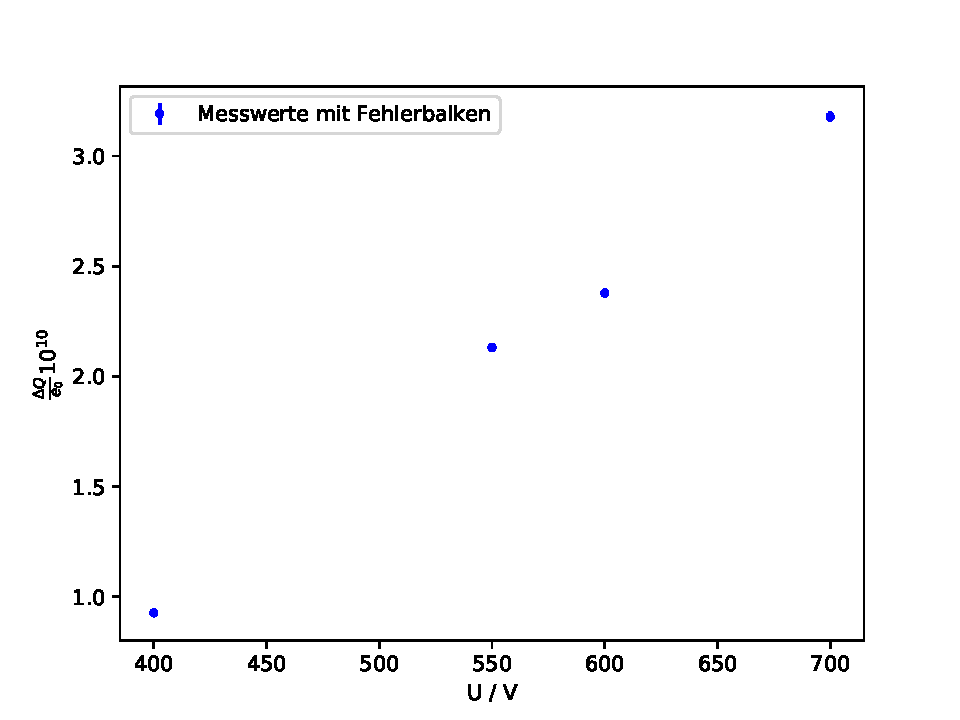
\includegraphics[scale=0.6]{3.pdf}
  \caption{Plot zur Darstellung des Verhältnisses zwischen Spannung und freigesetzter Ladungsmenge.}
  \label{abb3}
\end{figure}


\section{Diskussion}

Die im Experiment ermittelte prozentuale Steigung des linearen Fits an den Plateaubereich ist als sehr gering zu betrachten.Von daher
ist davon auszugehen, dass das Geiger-Müller-Zählrohr zuverlässig arbeitet. In der Literatur werden Steigungen innerhalb des Plateaubereichs bis
zu \SI{5}{\percent} toleriert \cite{Q2}.
Des Weiteren werden die grundsätzlichen Charakteristiken eines Geiger-Müller-Zählrohrs anhand der Grafik (siehe Abbildung \ref{abb1}) gut sichtbar.

\noindent Bei der Ermittlung der Totzeit fällt auf, dass sich deutliche Unterschiede zwischen den beiden Methoden abzeichnen.
In der Literatur \cite{Q2} sind keine exakten Angaben für die Totzeit kleiner Halogenzählrohre, wie dem im Versuch verwendeten, angeben.
Sie wird lediglich mit \SI{50}{\micro \second} bis \SI{100}{\micro \second} abgeschätzt.
Ausgehend von einem Wert von \SI{75}{\micro \second}, besteht bei der Ermittlung der Totzeit über die
zwei-Quellen-Methode eine prozentuale Abweichung von \SI{81,52}{\percent}. Die Prozentuale Abweichung von dem qualitativ ermittelten Wert
liegt hingegen bei \SI{176,67}{\percent}. Beide Bestimmungen sind daher als recht fehleranfällig zu betrachten.
Eine mögliche Fehlerquelle bei der Ermittlung durch die zwei-Quellen-Methode ist, dass beide Proben nicht den exakt gleichen Abstand vom
Glimmerfenster besitzen. Bei der qualitativen Bestimmung ist das exakte Ablesen des Oszillographen wahrscheinlich die größte Fehlerquelle.
Bei der Ermittlung der Erholungszeit ist die größte Schwierigkeit, die nur sehr kurz und mit einer hohen Frequenz aufblitzenden Kurven
wahrzunehemen. Deshalb kann der Abstand der beiden Maxima lediglich abgeschätzt werden.

\noindent Die Messungen der pro Teilchen freigesetzten Ladungsmengen ergaben plausible Werte und der lineare Zusammenhang zwischen den freigesetzten
Ladungsmengen und der angelegten Betriebsspannung ist trotz der wenigen Messwerte zu erahnen.
Hier bleibt zu erwähnen, dass bei wiederholtem Durchführen des Versuchs darauf zu achten ist, schon bei der Untersuchung der Charakteristik
des Zählrohrs, bei jeder Messung die entsprechenden Stromstärken zu notieren. Somit stehen zur Auswertung deutlich mehr Werte zur Verfügung,
was ein eindeutigeres Ergebnis liefern würde.



\newpage
\nocite{*}
\printbibliography
